\ifx\type\undefined
  \documentclass[10pt, t]{beamer}
  \setbeamertemplate{footline}[page number]
\else
  \documentclass[10pt]{article}
  \usepackage[margin=1in]{geometry}
\fi

\usepackage{amsmath}
\usepackage{amssymb}
\usepackage{amsthm}
\usepackage{cancel}
\usepackage{listings}
\usepackage{mathrsfs}
\usepackage{multirow}
\usepackage{soul}
\usepackage{stmaryrd}
\usepackage{tikz}
\usepackage{tikz-cd}
\usepackage{wrapfig}

\newtheorem*{algorithm}{Algorithm}
\newtheorem*{assumptions}{Assumptions}
\newtheorem*{conjecture}{Conjecture}
\newtheorem*{consequences}{Consequences}
\newtheorem*{exercise}{Exercise}
\newtheorem*{formalisation}{Formalisation}
\newtheorem*{proposition}{Proposition}
\newtheorem*{question}{Question}
\newtheorem*{remark}{Remark}

\ifx\type\undefined\else
  \newtheorem*{definition}{Definition}
  \newtheorem*{example}{Example}
  \newtheorem*{lemma}{Lemma}
  \newtheorem*{theorem}{Theorem}
\fi

\definecolor{keywordcolor}{rgb}{0.7, 0.1, 0.1}
\definecolor{tacticcolor}{rgb}{0.0, 0.1, 0.6}
\definecolor{commentcolor}{rgb}{0.4, 0.4, 0.4}
\definecolor{symbolcolor}{rgb}{0.0, 0.1, 0.6}
\definecolor{sortcolor}{rgb}{0.1, 0.5, 0.1}
\definecolor{attributecolor}{rgb}{0.7, 0.1, 0.1}
\def\lstlanguagefiles{lstlean.tex}
\lstset{language=lean}

\newcommand\A{\mathbb{A}}
\newcommand\C{\mathbb{C}}
\newcommand\F{\mathbb{F}}
\newcommand\G{\mathbb{G}}
\renewcommand\H{\mathbb{H}}
\newcommand\I{\mathbb{I}}
\newcommand\N{\mathbb{N}}
\renewcommand\P{\mathbb{P}}
\newcommand\Q{\mathbb{Q}}
\newcommand\R{\mathbb{R}}
\newcommand\Z{\mathbb{Z}}

\renewcommand\AA{\mathcal{A}}
\newcommand\BB{\mathcal{B}}
\newcommand\CC{\mathcal{C}}
\newcommand\DD{\mathcal{D}}
\newcommand\EE{\mathcal{E}}
\newcommand\FF{\mathcal{F}}
\newcommand\GG{\mathcal{G}}
\newcommand\HH{\mathcal{H}}
\newcommand\II{\mathcal{I}}
\newcommand\LL{\mathcal{L}}
\newcommand\MM{\mathcal{M}}
\newcommand\NN{\mathcal{N}}
\newcommand\OO{\mathcal{O}}
\newcommand\PP{\mathcal{P}}
\newcommand\RR{\mathcal{R}}
\renewcommand\SS{\mathcal{S}}
\newcommand\TT{\mathcal{T}}
\newcommand\XX{\mathcal{X}}

\renewcommand\aa{\mathfrak{a}}
\newcommand\cc{\mathfrak{c}}
\newcommand\dd{\mathfrak{d}}
\newcommand\ff{\mathfrak{f}}
\renewcommand\gg{\mathfrak{g}}
\newcommand\mm{\mathfrak{m}}
\newcommand\pp{\mathfrak{p}}
\newcommand\qq{\mathfrak{q}}
\renewcommand\ss{\mathfrak{s}}

\newcommand\LLL{\mathscr{L}}

\newcommand\ab{\mathrm{ab}}
\newcommand\Ab{\mathbf{Ab}}
\newcommand\Alg{\mathbf{Alg}}
\newcommand\Aff{\mathbf{Aff}}
\newcommand\Aut{\operatorname{Aut}}
\newcommand\Az{\mathrm{Az}}
\newcommand\Br{\operatorname{Br}}
\newcommand\BSD{\operatorname{BSD}}
\newcommand\ch{\operatorname{char}}
\newcommand\Cl{\operatorname{Cl}}
\newcommand\coker{\operatorname{coker}}
\newcommand\contr{\operatorname{contr}}
\newcommand\cris{\mathrm{cris}}
\renewcommand\d{\mathrm{d}}
\newcommand\Div{\operatorname{Div}}
\newcommand\dR{\mathrm{dR}}
\newcommand\EN{\operatorname{EN}}
\newcommand\End{\operatorname{End}}
\newcommand\ES{\operatorname{ES}}
\newcommand\et{\mathrm{\acute{e}t}}
\newcommand\Et{\mathbf{\acute{E}t}}
\newcommand\Ext{\operatorname{Ext}}
\newcommand\Fr{\operatorname{Fr}}
\newcommand\Frac{\operatorname{Frac}}
\newcommand\Gal{\operatorname{Gal}}
\newcommand\GL{\operatorname{GL}}
\newcommand\Gr{\mathrm{Gr}}
\newcommand\Hom{\operatorname{Hom}}
\newcommand\HT{\mathrm{HT}}
\newcommand\id{\operatorname{id}}
\newcommand\im{\operatorname{im}}
\newcommand\Ind{\operatorname{Ind}}
\renewcommand\inf{\operatorname{inf}}
\newcommand\inv{\operatorname{inv}}
\newcommand\Irr{\operatorname{Irr}}
\newcommand\Jac{\operatorname{Jac}}
\newcommand\lcm{\operatorname{lcm}}
\newcommand\Mat{\operatorname{Mat}}
\newcommand\Mod{\mathbf{Mod}}
\newcommand\Nm{\operatorname{Nm}}
\newcommand\nr{\mathrm{nr}}
\newcommand\NS{\operatorname{NS}}
\newcommand\Ob{\operatorname{Ob}}
\newcommand\ord{\operatorname{ord}}
\newcommand\op{\mathrm{op}}
\newcommand\PGL{\operatorname{PGL}}
\newcommand\Pic{\operatorname{Pic}}
\newcommand\Prob{\operatorname{Prob}}
\newcommand\Proj{\operatorname{Proj}}
\newcommand\PSh{\mathbf{PSh}}
\newcommand\Reg{\operatorname{Reg}}
\newcommand\res{\operatorname{res}}
\newcommand\rk{\operatorname{rk}}
\newcommand\Sch{\mathbf{Sch}}
\newcommand\Sel{\operatorname{Sel}}
\newcommand\Set{\mathbf{Set}}
\newcommand\sgn{\operatorname{sgn}}
\newcommand\Sh{\mathbf{Sh}}
\newcommand\SL{\operatorname{SL}}
\newcommand\Spec{\operatorname{Spec}}
\newcommand\supp{\operatorname{supp}}
\newcommand\Tam{\operatorname{Tam}}
\newcommand\Top{\mathbf{Top}}
\newcommand\tor{\operatorname{tor}}
\newcommand\tr{\operatorname{tr}}
\newcommand\tra{\operatorname{tra}}
\newcommand\WC{\operatorname{WC}}

\DeclareFontFamily{U}{wncyr}{}
\DeclareFontShape{U}{wncyr}{m}{n}{<->wncyr10}{}
\DeclareSymbolFont{cyr}{U}{wncyr}{m}{n}
\DeclareMathSymbol{\Sha}{\mathord}{cyr}{"58}

\newcommand{\function}[5][]{
  \if &#1&
    \begin{array}{rcl}
      #2 & \longrightarrow & #3 \\
      #4 & \longmapsto     & #5
    \end{array}
  \else
    \begin{array}{rcrcl}
      #1 & : & #2 & \longrightarrow & #3 \\
         &   & #4 & \longmapsto     & #5
    \end{array}
  \fi
}

\newcommand{\functions}[7][]{
  \if &#1&
    \begin{array}{rcl}
      #2 & \longrightarrow & #3 \\
      #4 & \longmapsto     & #5 \\
      #6 & \longmapsto     & #7 \\
    \end{array}
  \else
    \begin{array}{rcrcl}
      #1 & : & #2 & \longrightarrow & #3 \\
         &   & #4 & \longmapsto     & #5 \\
         &   & #6 & \longmapsto     & #7
    \end{array}
  \fi
}
\usetheme{singapore}
\title{Bridging Lean and the LMFDB}
\subtitle{Thematic Program on AI and Mathematics \\ Formalization, Theorem Proving and Reasoning}
\author{David Kurniadi Angdinata}
\institute{University of East Anglia}
\date{Wednesday, 15 July 2026}

\begin{document}

\frame{\titlepage}

\begin{frame}{The L-functions and modular forms database}

\begin{center}
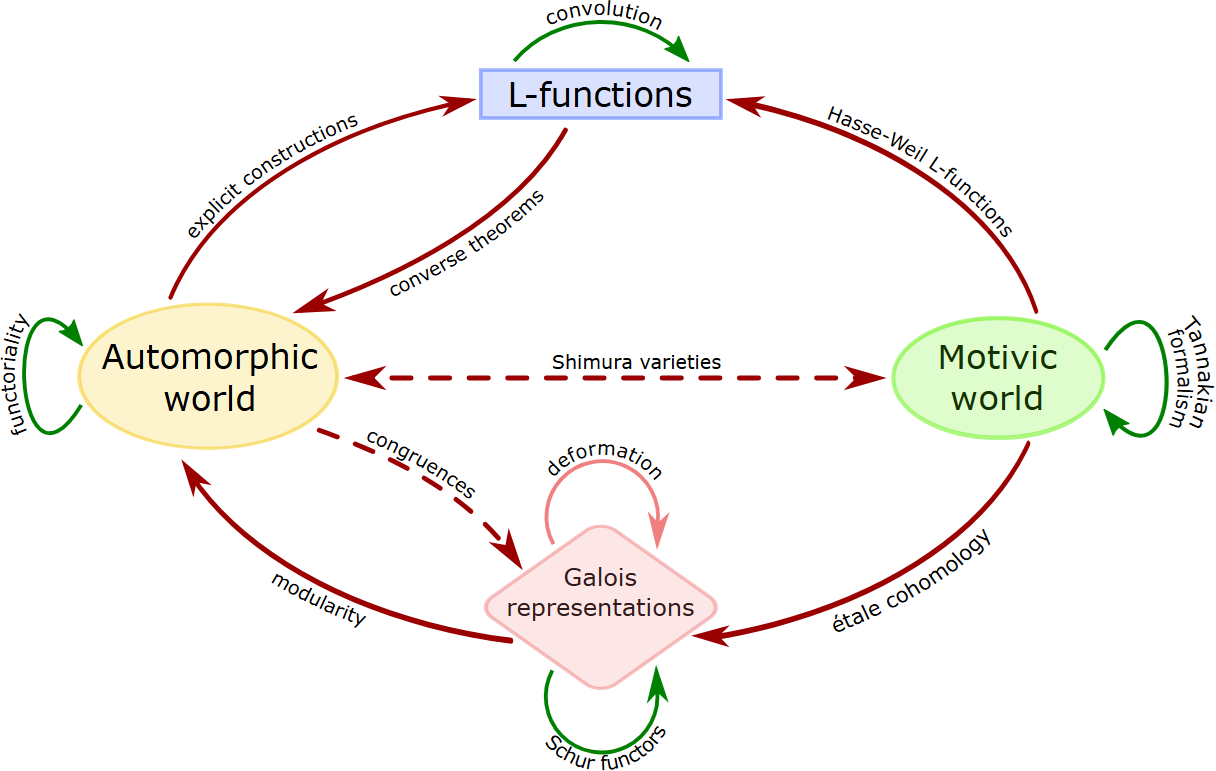
\includegraphics[width=\textwidth]{img/lmfdb.png}
\end{center}

\end{frame}

\begin{frame}{Objects in the LMFDB}

The LMFDB contains over 100 million objects with unique labels:
\begin{itemize}
\item 24m L-functions (rational and otherwise)
\item 850k modular forms (classical, Hilbert, Bianchi, Maass, and \emph{Siegel})
\item 42m varieties (elliptic curves over $ \Q $ and over number fields, genus two and higher genus curves over $ \Q $, and abelian varieties over $ \F_q $), Belyi maps, and \emph{modular curves}
\item 21m number fields and $ p $-adic fields
\item 1m abstract groups, Galois groups, Sato--Tate groups, and \emph{lattices}
\item 31m Dirichlet characters and Artin representations
\item \emph{60k hypergeometric motives}
\end{itemize}
There are also completeness and reliability considerations for each family.

\bigskip Each object has its own page, with data from computer algebra systems, and with links to the \textbf{knowl}edge database and other related objects.

\end{frame}

\begin{frame}{Scalable theorem proving via mathematical databases}

\begin{center}
\begin{tabular}{cc}

\includegraphics[height=0.2\textheight]{img/renaissancephilanthropy.jpg} & 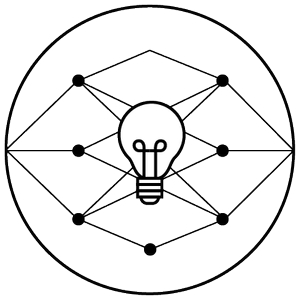
\includegraphics[height=0.2\textheight]{img/aiformathfund.jpg} \\
\end{tabular}
\end{center}

\bigskip

\begin{center}
\begin{tabular}{ccc}
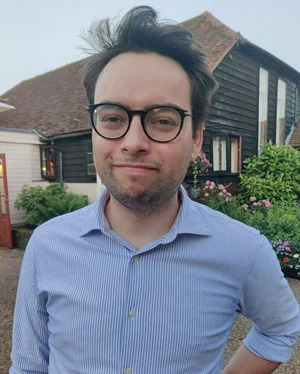
\includegraphics[height=0.4\textheight]{img/birkbeck.jpg} & 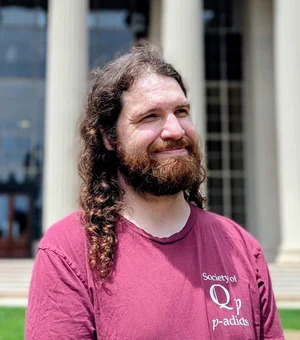
\includegraphics[height=0.4\textheight]{img/roe.jpg} & 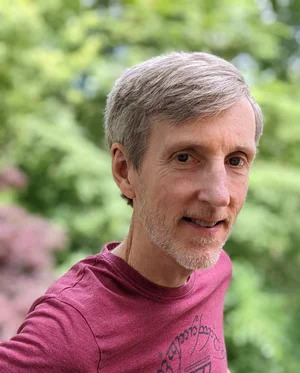
\includegraphics[height=0.4\textheight]{img/sutherland.jpg} \\
Chris Birkbeck & David Roe & Andrew Sutherland
\end{tabular}
\end{center}

\end{frame}

\begin{frame}{Objectives of the project}

The project has many closely-related objectives.

\bigskip On the side of the LMFDB:
\begin{itemize}
\item link the knowledge database to definitions in \texttt{mathlib}
\item add a command to preview the corresponding Lean statements
\item generate Lean proofs for simple or certifiable computations
\end{itemize}

\bigskip On the side of Lean and \texttt{mathlib}:
\begin{itemize}
\item add attributes to definitions that have LMFDB knowls
\item extend the property testing tactic to LMFDB objects
\item prove results assuming completeness and reliability of the LMFDB
\end{itemize}

\bigskip The \texttt{LeanBridge} repository hosts a rough blueprint, mostly on definitions for number fields, elliptic curves over $ \Q $, and classical modular forms.

\end{frame}

\begin{frame}{Workshop in Norwich}

A workshop with over 50 participants was held in the University of East Anglia from Monday, 29 June 2026 to Friday, 3 July 2026.

\begin{center}
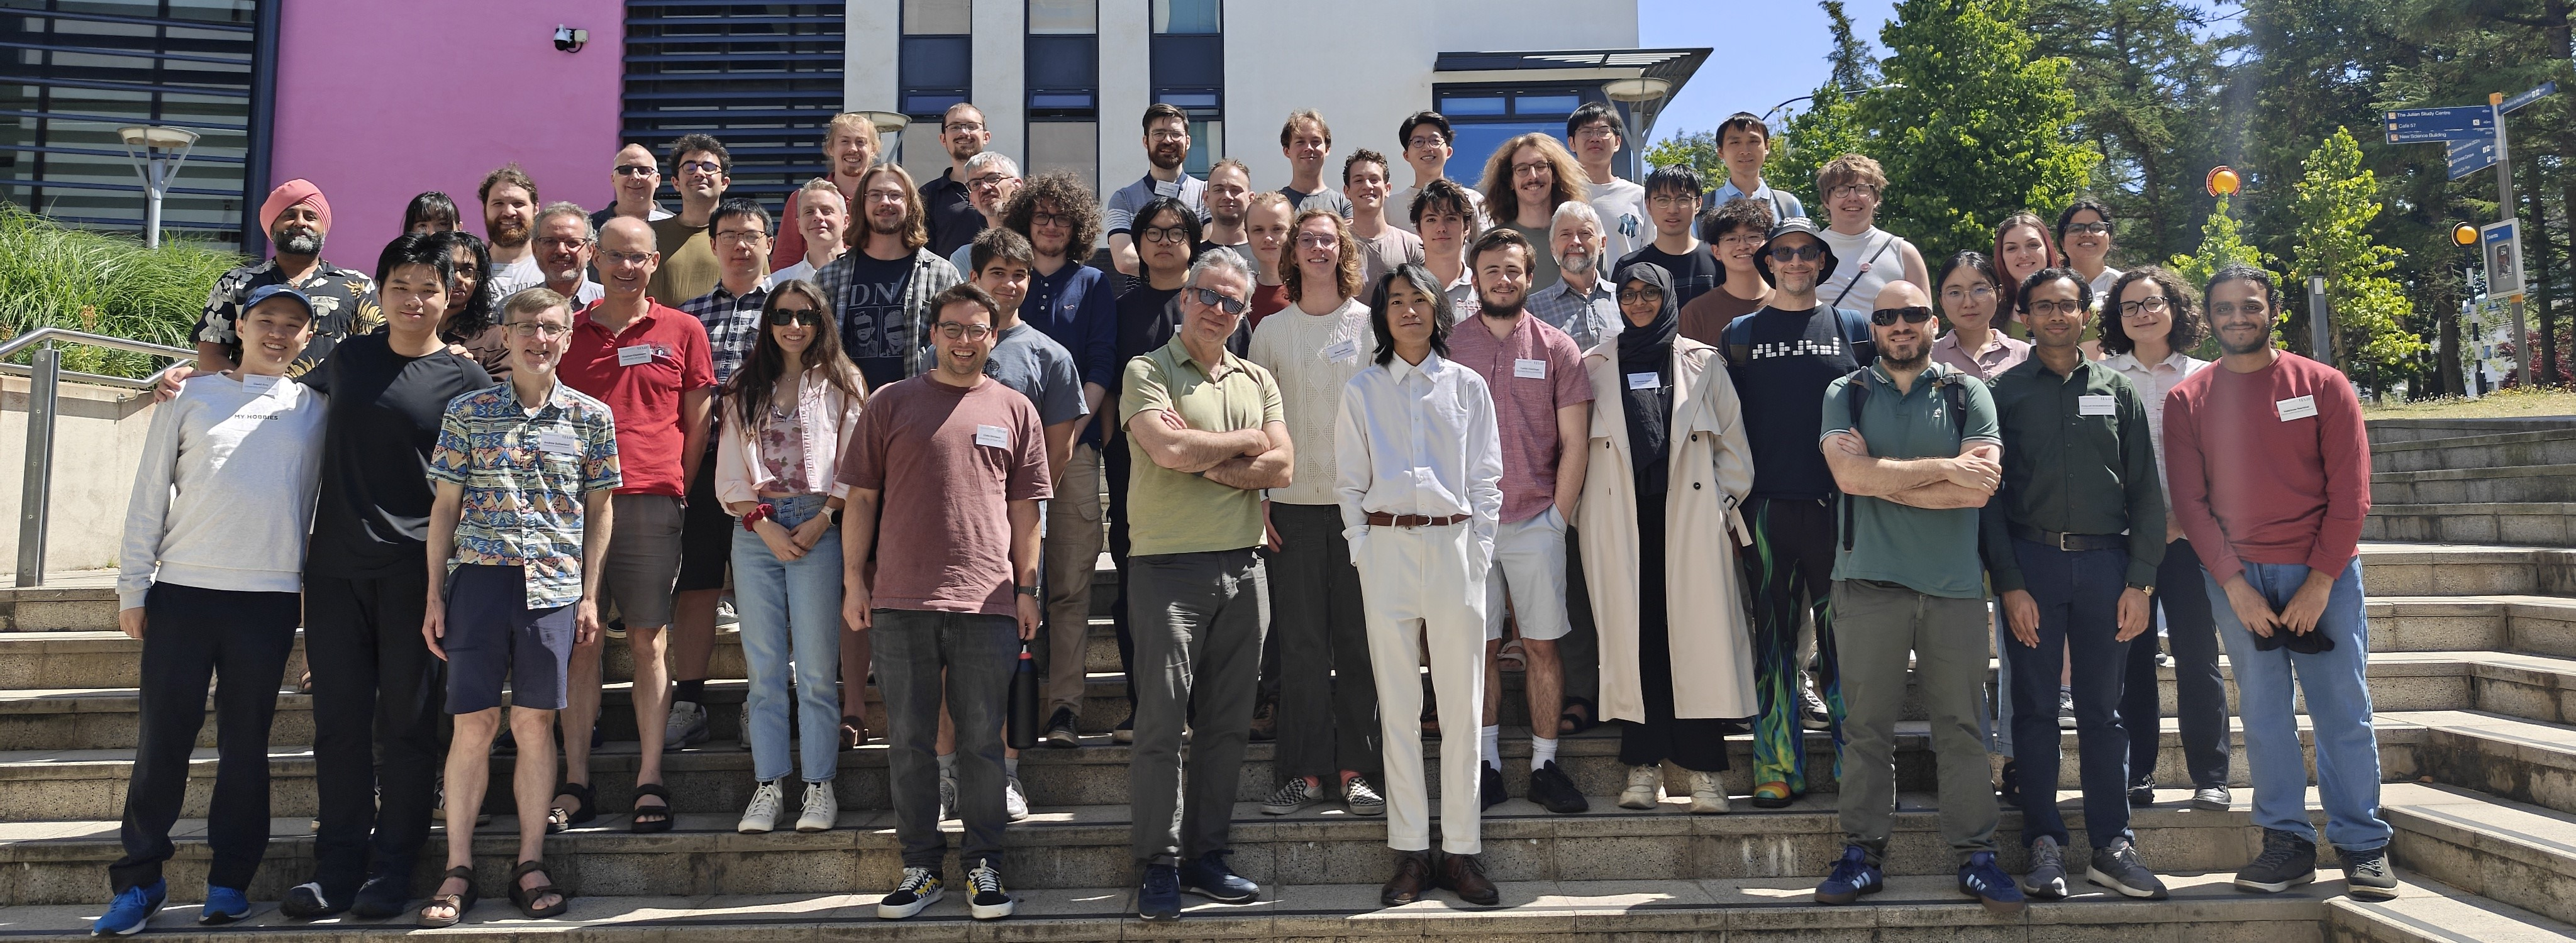
\includegraphics[width=\textwidth]{img/lean-lmfdb.jpg}
\end{center}

\bigskip There will be another workshop in the Massachusetts Institute of Technology from Monday, 25 January 2027 to Friday, 29 January 2027.

\end{frame}

\begin{frame}{Number fields}

A large group worked on certifying the class number formula
$$ \lim_{s \to 1} ((s - 1) \cdot \zeta_K(s)) = \frac{2^{r_1} \cdot (2\pi)^{r_2} \cdot \Reg_K \cdot h_K}{w_K \cdot \sqrt{|D_K|}}, $$
which was formalised in \texttt{mathlib} by Xavier Roblot in May 2025.
\begin{itemize}
\item \emph{Anne Baanen}, \emph{Sander Dahmen}, and Alain Chavarri Villarello had previously certified many invariants of $ \OO_K $, including $ D_K $ and $ h_K $.
\item David Ledvinka had a tactic for interval arithmetic.
\item Bhavik Mehta and \emph{Heather Macbeth} had previous results on isolation of roots and error bounds of matrix determinants.
\item Chris Birkbeck computed an error bound for $ \lim_{s \to 1} ((s - 1) \cdot \zeta_K(s)) $.
\item Along with everyone else above, Barinder Banwait, Thomas Browning, Stephan Elsenhans, Xavier G\'en\'ereux, Artie Khovanov, and Arend Mellendijk computed an error bound for $ \Reg_K $.
\end{itemize}
They verified the class number formula for one sextic number field.

\end{frame}

\begin{frame}{Elliptic curves}

In contrast, \texttt{mathlib} has little on elliptic curves, mostly formalised by Junyan Xu and me. This includes the group law, the basics of division polynomials, and parts of the multiplication-by-$ n $ formula.
\begin{itemize}
\item Chris Birkbeck and I formalised the Lutz--Nagell theorem, with ongoing work to compute torsion subgroups over $ \Q $.
\item \emph{Michael Stoll} formalised heights over number fields, with potentially ongoing work on the Mordell--Weil theorem.
\item Riccardo Brasca, Richard Hill, and Edison Xie continued their work on continuous cohomology and defined the Tate--Shafarevich group.
\item Bhavik Mehta certified lower rank bounds, including the rank $ \ge29 $ Elkies--Klagsbrun curve discovered in 2024, and even found an error in the rank $ \ge21 $ Nagao--Kouya curve discovered in 1994.
\item Håvard Damm-Johnsen, Zachary Feng, and Jane Shi added the Lean command for curve and isogeny class pages in the LMFDB.
\end{itemize}

\end{frame}

\begin{frame}{Modular forms}

Similarly, \texttt{mathlib} has little on modular forms, mostly formalised by Chris Birkbeck and David Loeffler. This includes actions on $ \H $, classical Eisenstein series, q-expansions, and finite dimensionality for $ \SL_2(\Z) $.
\begin{itemize}
\item Chris Birkbeck maintains the massive \texttt{AINTLib/LeanModularForms} repository, which contains the valence formula for $ \SL_2(\Z) $ and the strong multiplicity one theorem for newforms with nebentypus.
\item David Loeffler continued his work on L-functions for modular forms.
\item Ramin Takloo-Bighash and Samuel Yin formalised duality for cusp forms with nebentypus and coefficient fields of Hecke eigenforms.
\item Wenrong Zou and James Kiln formalised Eisenstein series with nebentypus and computed their q-expansions.
\item William Coram, John Cremona, Nicola Falciola, Sayeb Salam, and Samuel Yin worked on uniformisation theorems over $ \C $ and $ \Q_p $.
\end{itemize}

\end{frame}

\begin{frame}{Miscellaneous}

Numerous other projects!
\begin{itemize}
\item Bhavik Mehta developed the \texttt{lookup} tactic for Galois groups, number fields, elliptic curves, and modular forms.
\item \emph{Mario Carneiro}, \emph{James Davenport}, and Michail Karatarakis developed kernel-reducible computable multivariate polynomials.
\item Yunfei Li and Jiaqi Wang worked on an interface for $ p $-adic fields and their ramification theory for finite extensions.
\item Peiran Wu formalised Gassmann equivalences of subgroups.
\item Justus Springer and Peiran Wu worked on affine group schemes.
\item Ammara Ansari, Giovanna De Lauri, Vaishnav Nambiar, Yufei Qian, Pratyush Venkatakrishnan, and Xindi Yang worked on lattices and kissing numbers, supervised by Riccardo Brasca and Kevin Buzzard.
\end{itemize}

\end{frame}

\end{document}